
%\textbf{Anschluss:} 

\begin{figure}[ht]
  \centering
  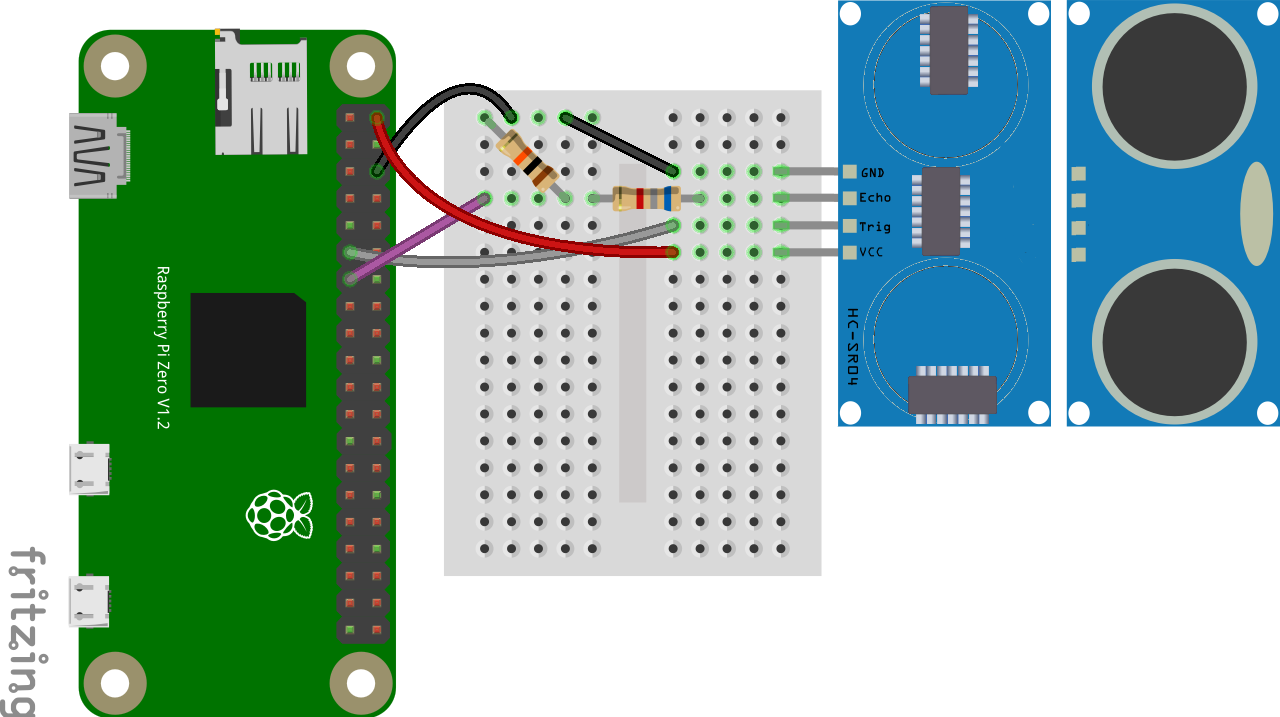
\includegraphics[scale=0.25]{images/HC-SR04_Steckplatine.png}	
  %	\caption{}
  \label{DHT22_Steckplatine}
\end{figure}

%\textbf{Schaltplan:} 

\begin{figure}[ht]
	\centering
	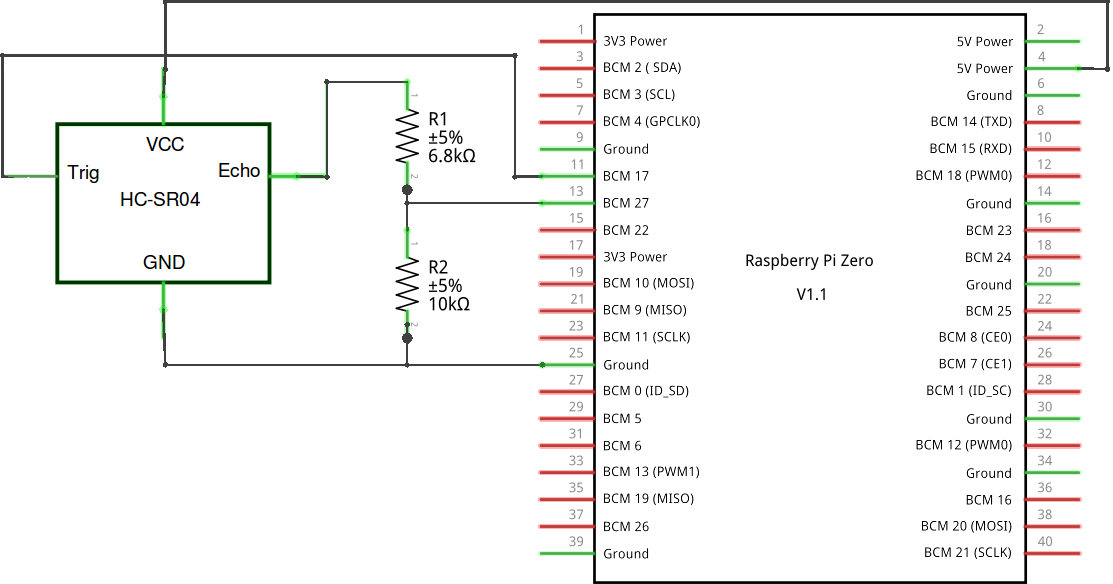
\includegraphics[scale=0.25]{images/HC-SR04_Schaltplan.png}	
	%	\caption{}
	\label{DHT22_Steckplatine}
\end{figure}

\textbf{C:} 

\begin{console}
	git clone https://github.com/mstroh76/HC-SR04Sensor
	cd HC-SR04Sensor
	geany project.geany & 
\end{console}

\textbf{C\#:}

\begin{console}
git clone https://github.com/chirndler/wiringpi.net.sensors.git
cd wiringpi.net.sensors
xbuild /p:Configuration=Release wiringpi.net.sensors.sln
cd bin/Release/
sudo mono wiringpi.net.sensors.sample.exe 2
\end{console}

\textbf{Python:}

\lstset{language=Python, caption=, 
        label=HCSR04Program, frame=single, basicstyle=\ttfamily
	      \footnotesize, breakatwhitespace=false, showstringspaces=false, 
        showtabs=false, tabsize=2 }
\lstinputlisting{source/HC_SR04.py}

